%# -*- coding: utf-8 -*-
% !TEX encoding = UTF-8 Unicode
\RequirePackage{fixltx2e}
\documentclass[aps,pre,12pt,preprint,onecolumn,showpacs,showkeys,UTF8]{revtex4-1}
\usepackage{ctex}
\usepackage{mathrsfs}
\usepackage{setspace,dcolumn}
\usepackage{subfigure}
\usepackage{graphicx,psfrag,epsfig}
\usepackage[font=small,format=plain,labelfont=bf,textfont=it,justification=raggedright,singlelinecheck=false]{caption}
\usepackage{amsmath,amsfonts,amssymb,amsthm,bm,upgreek}
\usepackage{geometry}
\usepackage[mathscr]{eucal}
\usepackage{titlesec}
\usepackage{tabularx}
\titleformat{\section}{\bf\fangsong\zihao{4}}{\thesection}{0.75em}{}
\geometry{top=2.54cm,bottom=2.54cm,left=3cm,right=3cm}
\renewcommand\appendixname{附录}
\renewcommand\abstractname{}%摘要
\renewcommand\tablename{表}
\renewcommand\figurename{图}
\makeatletter
\def\@keys@name{\songti\zihao{-4}{\bf 关键词:}}
\def\Received@name{\zihao{-5}{接收} }
\def\Revised@name{\zihao{-5}{修订} }
\def\Accepted@name{\zihao{-5}{采纳} }
\def\Published@name{\zihao{-4}{发表} }
\makeatother
\linespread{1.6}
\renewcommand{\labelenumi}{\alph{enumi}.}
\leftmargini=20mm

\begin{document}

\title{\bf\heiti\zihao{3}符合测量\vspace{15mm}}
\author{\fangsong 乔颢\vspace{2mm}}
\affiliation{\songti\zihao{-4}北京大学物理学院2011级2班~~~~学号:1100011354 \vspace{2mm}}
\keywords{符合测量,钴,放射活度}
\email{1993422qsh@gmail.com; 18600200672}
\begin{abstract}
	\vspace{10mm}
	\begin{spacing}{1.5}
		\songti\zihao{-4}
		这个实验利用了$^{60}$Co在衰变过程中会释放出一个$\beta$粒子和两个$\gamma$光子的现象,利用$\beta-\gamma$符合测量得到了样品的绝对活度。得到的数值为$D=(5.4\pm0.2)\times10^5 min^{-1}$。理论值为$D=5.63\times10^5 min^{-1}$。实验结果与理论符合较好。
	\end{spacing}
\end{abstract}

\maketitle

\section{引言}
符合测量技术是现代核物理实验的基本实验技术之一,在各个领域都有着广泛的应用。因为其作为一种排除偶然因素,真是测定事件的实验手段,所以其在反应物能量角分布,核衰变机制研究中广泛应用,已经成为了实现多参数测量的必不可少的手段。

历史上的符合测量最初是用语宇宙射线的研究,而后逐渐推广开来。这个实验的目的是学习符合测量的基本方法,测量符合装置的分辨时间,同时使用$\beta-\gamma$符合测量$^{60}$Co的放射性活度。

符合测量中测量的是符合事件发生的次数。所谓的符合事件是指有两个或者两个以上同时发生的事件。符合法就是利用符合电路筛选出符合事件。但是探测中除了存在因果关系的符合输出外,也存在着偶然间发生的符合事件。前者被称作真符合,后者被称作偶然符合。

而偶然符合则可以通过以下的方式计算出来。设一个事件经过符合装置处理形成了一个宽度为$\tau$的矩形脉冲信号,同时符合电路中第一个符合道探测器记录的单位时间平均计数为$m_1$,第二道为$m_2$。则很容易得到,对于第一个符合道探测到的事件,如果第二个符合道在其前后$\tau$的时间内也探测到了符合事件,则这就引起了一个偶然符合,所以其平均的计数为:
\begin{equation}
	m_{rc}=2m_1m_2\tau
\end{equation}
如果两个脉冲的宽度不相等,则有
\begin{equation}
	m_{rc}=m_1m_2(\tau_1+\tau_2)
\end{equation}
此时的符合时间为$\tau=\frac{1}{2}(\tau_1+\tau_2)$。

$^{60}$Co的半衰期为5.27年,衰变时其放出一个$\beta$粒子之后变成了激发态的$^{60}$Ni,然后在$10^{-11}$时间内放出两个$\gamma$光子跃迁回基态。这个实验则是利用放射源的$\beta-\gamma$符合来测量其放射活度。其活度可以由以下公式给出:
\begin{equation}
	D=\frac{m_{1\beta}m_{2\gamma}}{m_{\beta\gamma}}
\end{equation}
其中$m_{1\beta}$为$\beta$粒子引起的计数,$m_{2\gamma}$为$\gamma$粒子引起的,分母则是两者的符合计数。考虑到本地计数等等的影响,上公式可以改写为:
\begin{equation}
	D=\frac{(m_1-m_1')(m_2-m_{2b})}{m_c-m_c'-2\tau(m_1-m_1')\cdot m_2}
\end{equation}
式子中$m_1,m_1'$分别为有无$\beta$粒子的时候$\beta$探测器的计数。$m_2,m_{2b}$为$\gamma$探测器对于样品的计数以及本底的计数。$m_c,m_c'$为有无$\beta$粒子时候的符合计数。

\section{实验}
\subsection{实验装置}
\begin{figure}[h]
	\begin{center}
		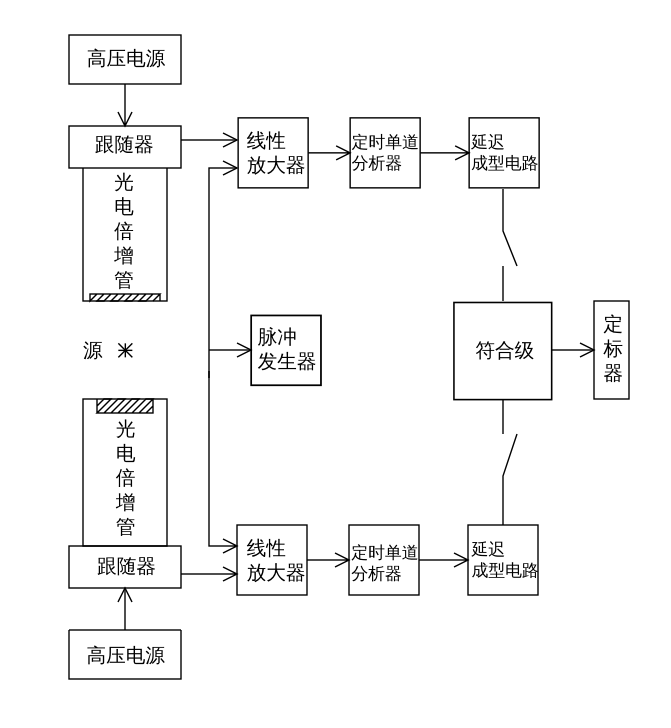
\includegraphics[width=0.7\textwidth]{pic1.png}
		\caption{\label{fig:exp1}符合测量元器件示意图}
	\end{center}
\end{figure}

实验装置如图所示,源发射出$\beta,\gamma$两种粒子,被两个探头所接收,探头通过闪烁体将粒子的动能吸收转化为光子并经过光电倍增管转化为电信号,输入到线性放大器里。线性放大器对于信号进行初步的放大后将信号输入到单道。单道筛选出合适的幅度的信号并将其转换为方波信号。两道信号进入符合单元,符合后由定标器定标计数。
\subsection{实验步骤以及数据}

按照上文示意图所示连接好电路图,给探头加上高压,然后并不连入电路而是将脉冲信号发生器给出的信号作为标准信号输入,从而求出符合电路的电子学符合时间。调整的脉冲宽度在$0.6\mu s$,此时$\gamma$通道的放大倍数为177倍,$\beta$为190倍。计数时间为4s,得到的数据如下:
\begin{center}
	\begin{table}[h]
		\caption{电子学分辨时间测量的数据图。放大倍数177,190。测量时间4s}
		\begin{tabularx}{6cm}{XX}
			\hline
			\hline
			延迟时间/$\mu s$&计数\\
			\hline
3.6	&	0	\\
3.7	&	0	\\
3.8	&	0	\\
3.9	&	38752	\\
4	&	38753	\\
4.1	&	38753	\\
4.2	&	38754	\\
4.3	&	38753	\\
4.4	&	38747	\\
4.5	&	38753	\\
4.6	&	38753	\\
4.7	&	38753	\\
4.8	&	38753	\\
4.9	&	38753	\\
5	&	38753	\\
5.1	&	38753	\\
5.2	&	0	\\
5.3	&	0	\\

			\hline
			\hline
		\end{tabularx}
	\end{table}
\end{center}
对数据做图可以得到以下的结果:
\begin{figure}[h]
	\begin{center}
		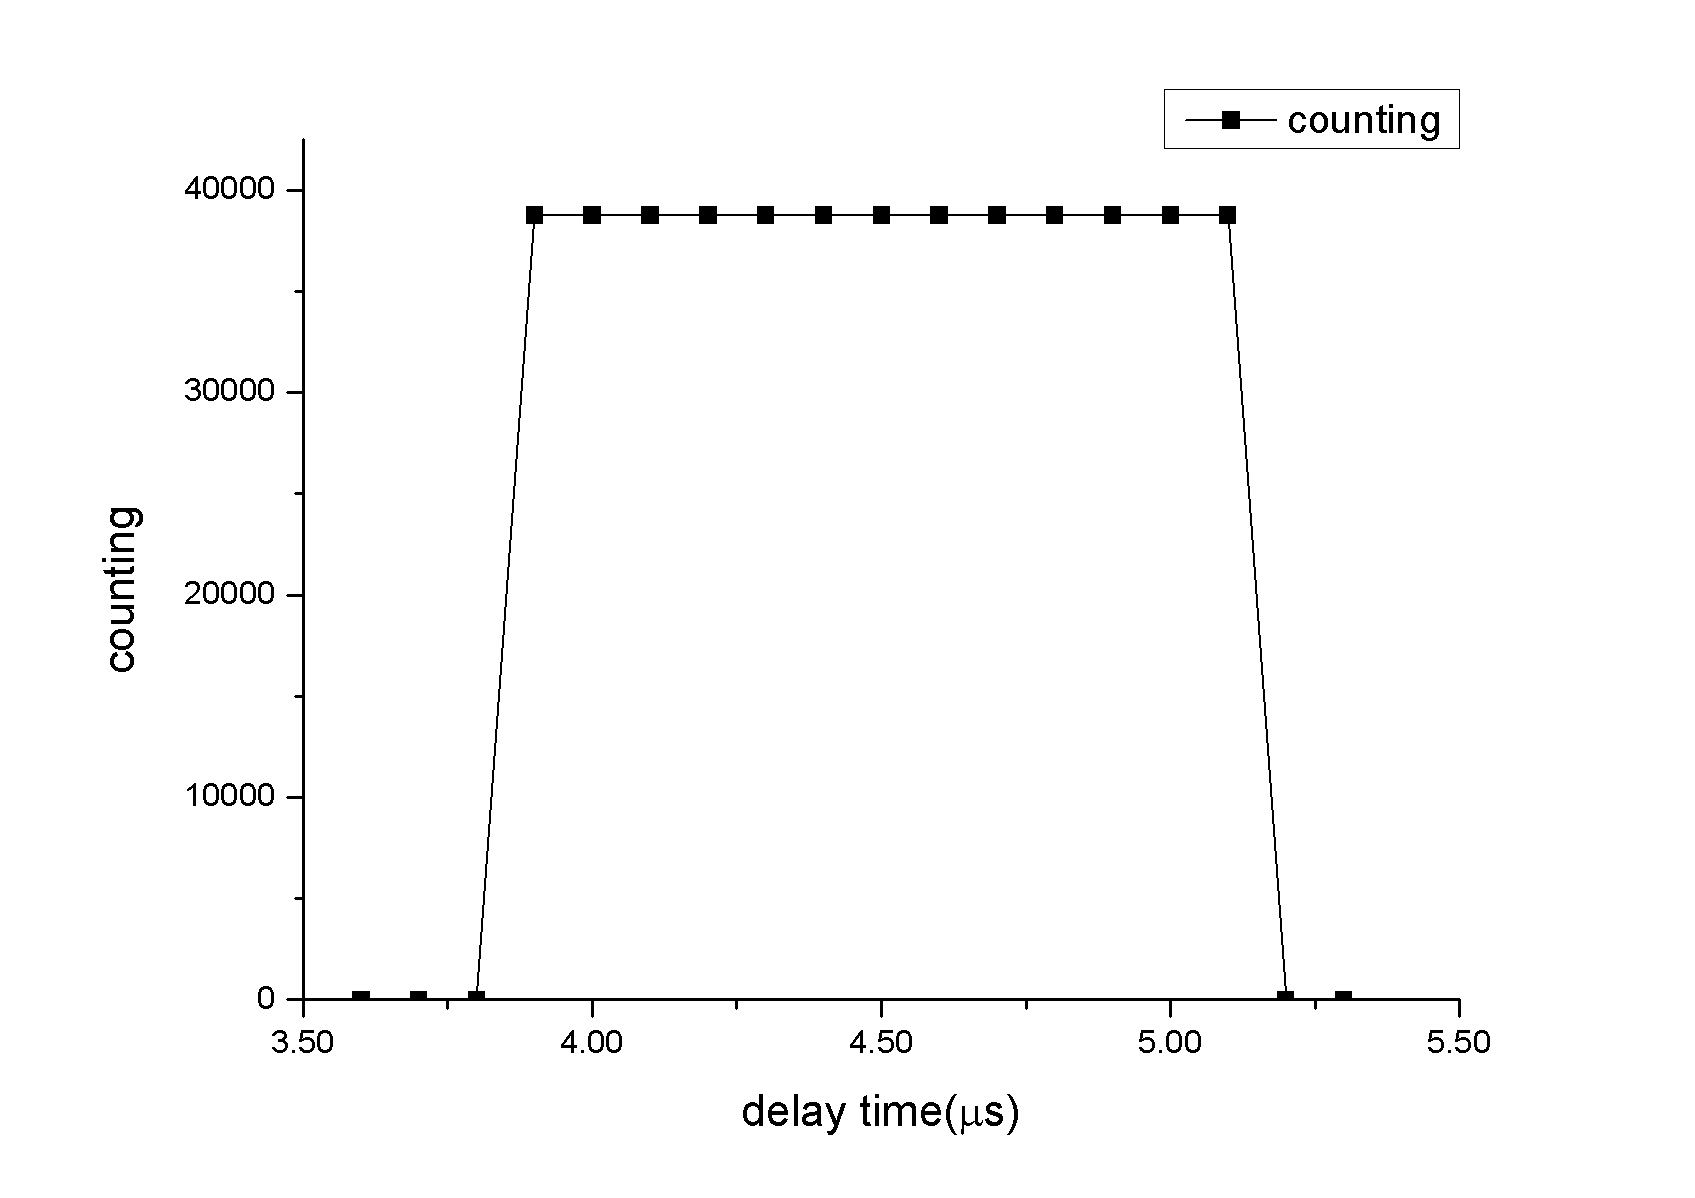
\includegraphics[width=0.7\textwidth]{pic2.png}
		\caption{\label{fig:exp1}电子学分辨时间测量的数据图}
	\end{center}
\end{figure}

可以看出,在以信号发生器作为发生源的时候,给出的电子学符合事件也就是给定脉冲宽度的两倍$1.2\mu s$。图像十分的整齐平滑,跟预期完全一致。

接下来便是测量真是样品的符合计数,并由此给出符合电路的物理分辨时间。将探测器的信号输入到符合电路,可以得到以下的数据:
\begin{center}
	\begin{table}[h]
		\caption{物理学分辨时间测量的数据图。放大倍数176,58。测量时间60s}
		\begin{tabularx}{12cm}{XXXX}
			\hline
			\hline
			延迟时间/$\mu s$&计数&延迟时间/$\mu s$&计数\\
			\hline
3.5	&	240	&	4.7	&	8689	\\
3.6	&	303	&	4.8	&	8475	\\
3.7	&	440	&	4.9	&	8408	\\
3.8	&	708	&	5	&	8443	\\
3.9	&	1012	&	5.1	&	7972	\\
4	&	1715	&	5.2	&	7590	\\
4.1	&	2632	&	5.3	&	6927	\\
4.2	&	4726	&	5.4	&	5982	\\
4.3	&	7039	&	5.5	&	3733	\\
4.4	&	8479	&	5.6	&	1253	\\
4.5	&	8684	&	5.7	&	178	\\
4.6	&	8691	&	\\			
			\hline
			\hline
		\end{tabularx}
	\end{table}
\end{center}

做图得到下面的图片
\begin{figure}[h]
	\begin{center}
		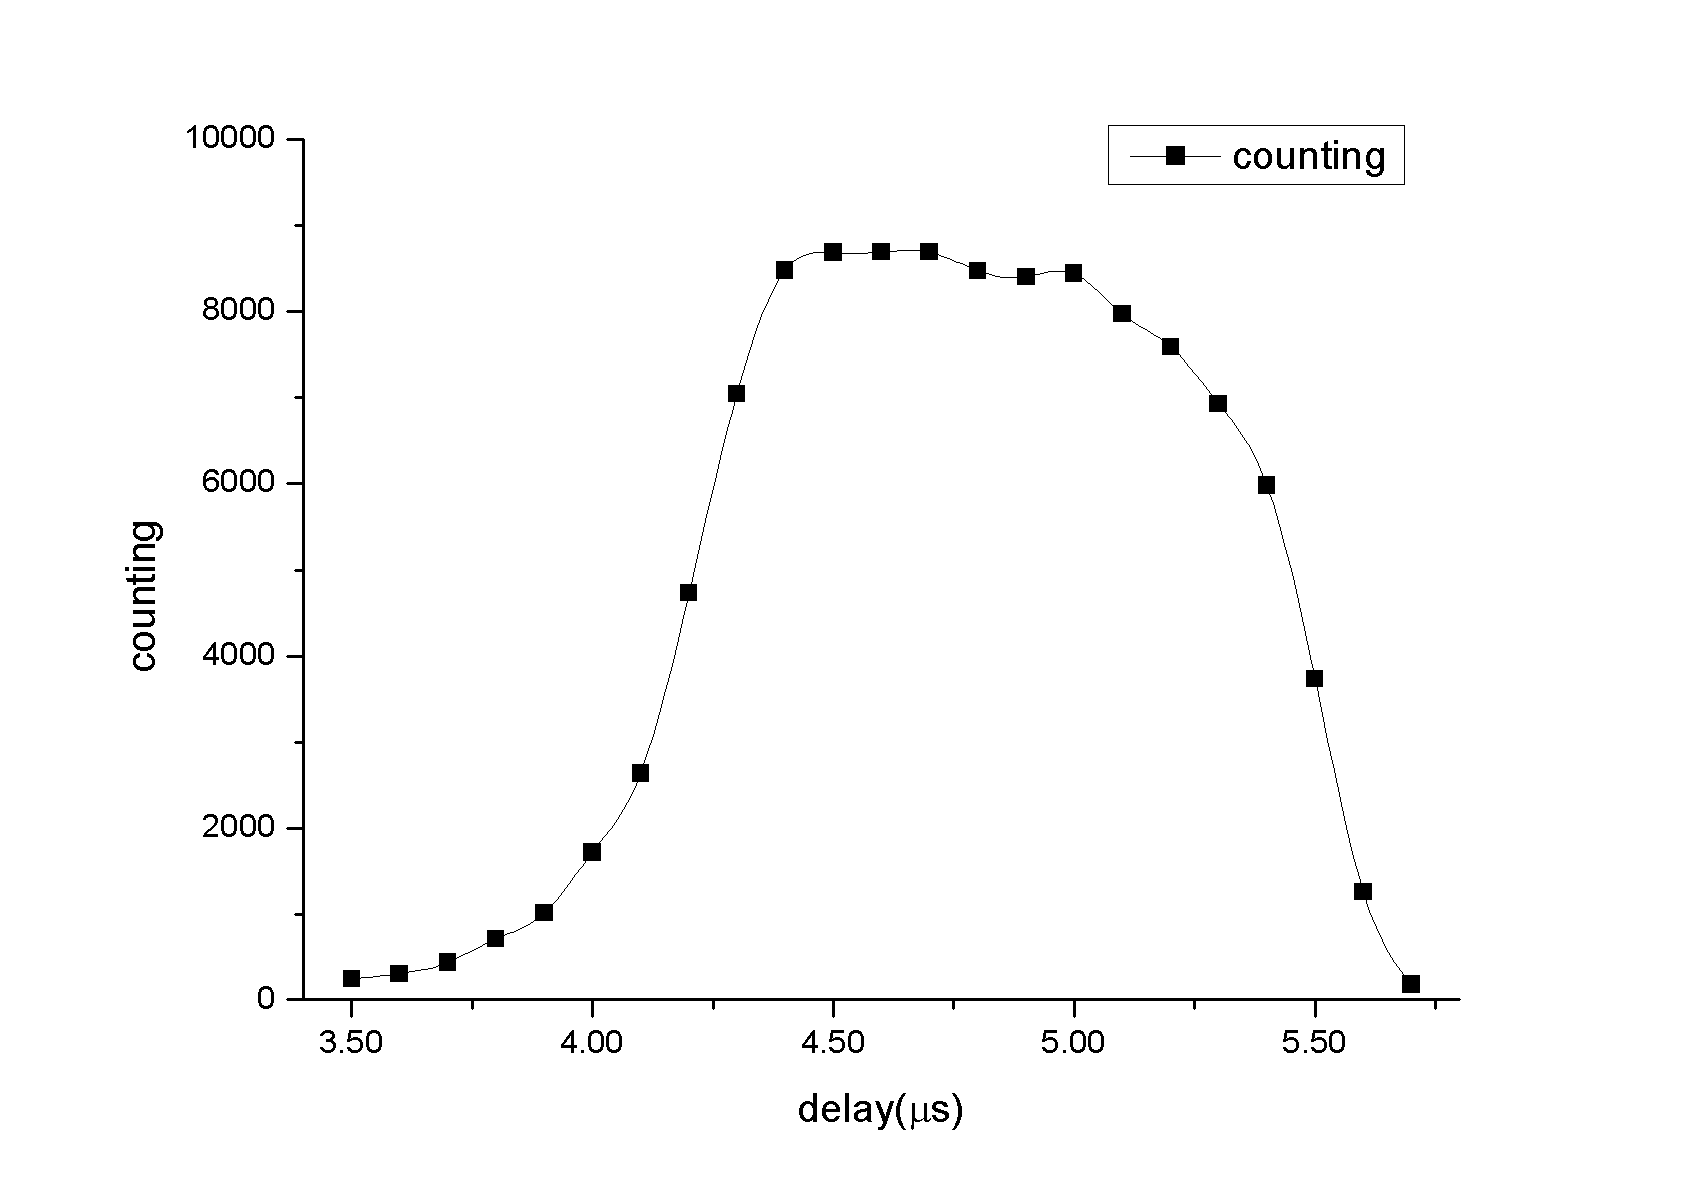
\includegraphics[width=0.7\textwidth]{pic3.png}
		\caption{\label{fig:exp1}物理学分辨时间测量的数据图}
	\end{center}
\end{figure}

可以看出他不在是像电子学分辨时间平直曲线。而且与理论相比较不是一个对称的结果。这一点不太能够理解,可能是因为探测仪的脉冲有时间离散。从上图中可以读出半高宽,可以得到物理学分辨时间$0.64\pm 0.02\mu s$。这里面的误差是由读数因素估测给出的。

随后便是计算钴源的活度。测量得到的数据如下:
\begin{center}
	\begin{table}[h]
		\caption{钴源活度的测量}
		\begin{tabularx}{12cm}{XXXXX}
			\hline
			\hline
			测量值&第一次计数&第二次计数&第三次计数&平均值\\
			\hline	
			$m_1$&48880&48694&48819&48798\\
			$m_2$&94270&94273&94234&94259\\
			$m_c$&8581&8658&8510&8583\\
			$m_1'$&5482&5608&5696&5595\\
			$m_c'$&951&933&976&953\\
			$m_2'$&772&784&813&790\\
			\hline
			\hline
		\end{tabularx}
	\end{table}
\end{center}

带入公式即可计算出D的值为$D=5.353\times10^5 min^{-1}$。误差由以下式子给出:
\begin{equation}
	\sigma_D=\sqrt{(\frac{\partial D}{\partial m_1}\sigma_{m_1})^2+(\frac{\partial D}{\partial m_c}\sigma_{m_c})^2+(\frac{\partial D}{\partial m_2}\sigma_{m_2})^2+(\frac{\partial D}{\partial m_1'}\sigma_{m_1'})^2+(\frac{\partial D}{\partial m_c'}\sigma_{m_c'})^2+(\frac{\partial D}{\partial m_{2b}}\sigma_{m_{2b}})^2+(\frac{\partial D}{\partial \tau}\sigma_{tau})^2}
\end{equation}

给出其结论为 $D=(5.4\pm0.2)\times10^5 min^{-1}$。可以看到误差还是不小的,其中误差的一般来自于物理分辨时间的测量,所以可以考虑使用更好的做图方式给出更精确的物理分辨时间。

通过理论计算可以得到实验中的源的活性为$D=5.63\times10^5 min^{-1}$。试验结果可以说基本符合了理论的测量。相对偏差在4.9\%。测量结果偏小的原因可鞥时因为放大倍数调整的不是十分合理以至于一些数据偏差很大。

\section{结论}

本实验通过$\beta-\gamma$符合测量测定$^{60}$Co的活性,得到的结果是
\begin{equation}
	D=(5.4\pm0.2)\times10^5 min^{-1}
\end{equation}
与理论之相比偏小。可能是由于参数调整的原因造成的。

\section{致谢} 
感谢楼建玲老师的指导,以及贾春燕,冉书能老师的技术支持。


\begin{thebibliography}{}
	\bibitem{Book} 吴思成,王祖铨~2010 近代物理实验(第三版)(北京:高等教育出版社)第274页.%
%
\end{thebibliography}

\clearpage
\appendix
\section{思考题}

1、实验中采用闪烁计数器,将粒子的能量吸收转化为光信号,并通过光电倍增管形成电信号,经过下游电路筛选整形等处理后计数。$\beta$计数用$\beta$探头测量值与加上铝板遮住的值的差即可。$\gamma$用样品值减去本底值即可。

2、固定一路后在示波器目测另外一路产生的信号,调整延迟从目测符合发生次数较少到最多期间即可确定出测量范围。这时候测量较快。

3、由公式可以得到要求$\tau < \frac{1}{20D}$ 即可。代入活度就可以得到分辨时间。

4、不可太厚影响$\gamma$粒子的探测,也不能太薄以至于不能完全阻挡$\beta$粒子。5mm左右是一个比较合适的值。

5、可以使用双$\gamma$测量,不过因为光子之间有一定的角度,所以可能需要矫正。有最后计算为$D=\frac{m_{1\gamma}m_{2\gamma}}{2m_{2\gamma}}$。推导过程中要用到认为放射的光子各项同性,向各个方向发射的概率是一样的。同时也要求探头的性能一致,这样才可以使得探头接收到的光子的概率相同从而能使用上述公式。

\section{记录本}
已经检查了,就不上传了。

\end{document} 
